\documentclass{beamer}
\usepackage{listings}
\usepackage{tikz}
\usepackage{mathtools}
\usetikzlibrary{arrows}

\title[Effprog]%(optional, only for long titles)
{185.190 Effiziente Programme}
\subtitle{Aufgabe: Hash-Tabelle}
\author{Berger G., Hotz-Behofsits C., Reisinger M., Schmidleithner T.}
\date{WS12/13}
\subject{Informatik}

\lstset{breakatwhitespace,
language=C,
keywordstyle=\color{blue},
stringstyle=\color{red},
commentstyle=\color{gray},
columns=fullflexible,
keepspaces,
breaklines,
tabsize=3,
showstringspaces=false,
extendedchars=true}

\newcommand{\success}[1]{\textcolor{green}{#1}}
\newcommand{\fail}[1]{\textcolor{red}{#1}}

\tikzset{
  treenode/.style = {align=center, inner sep=3pt, text centered,
    font=\sffamily},
  arn_n/.style = {treenode, black, font=\sffamily, text width=5.5em, inner sep=3pt},% arbre rouge noir, noeud noir
  arn_r/.style = {treenode, red, text width=5.5em, inner sep=3pt},% arbre rouge noir, noeud rouge
  arn_x/.style = {treenode, green, text width=5.5em, inner sep=3pt }% arbre rouge noir, nil
}

\begin{document}
	% Inlining
	\defverbatim[colored]\sInlining{%
\begin{lstlisting}[tabsize=8,basicstyle=\ttfamily]
inline unsigned long hash(char *addr, size_t len);
inline void insert(char *keyaddr, size_t keylen, int value);
inline int lookup(char *keyaddr, size_t keylen);
\end{lstlisting}}


	% Main loop
	\defverbatim[colored]\duploop{%
\begin{lstlisting}[tabsize=4,basicstyle=\ttfamily]
for (i=0; i<10; i++) {
	for (p=input2.addr, endp=input2.addr+
		input2.len; p<endp; ) {
		nextp=memchr(p, '\n', endp-p);
		if (nextp == NULL)
			break;
		r = ((unsigned long)r) * 2654435761L + lookup(p, nextp-p);
		r = r + (r>>32);
		p = nextp+1;	
	}
}
\end{lstlisting}}


	% differenzengleichung
	\defverbatim[colored]\diffgleichung{%
\begin{lstlisting}[tabsize=4,basicstyle=\ttfamily]
r = ((unsigned long)r) * 2654435761L + lookup(p, nextp-p);
r = r + (r>>32);

\end{lstlisting}}

	% Lineares Sondieren
	\defverbatim[colored]\sLinear{%
\begin{lstlisting}[tabsize=8,basicstyle=\ttfamily\footnotesize]
void insert(char *keyaddr, size_t keylen, int value) {
    struct hashnode **l;
    int startPosition = hash(keyaddr, keylen) & (HASHSIZE-1);
    int position = startPosition;
    do {
        l = &ht[position];
        position = (position + 1) % HASHSIZE;
    } while(*l != NULL && position != startPosition);

    if (*l == NULL) {
        struct hashnode *n = malloc(sizeof(struct hashnode));
        n->keyaddr = keyaddr;
        n->keylen = keylen;
        n->value = value;
        *l = n;
    }
}
\end{lstlisting}}

	% Quadratisches Sondieren
\defverbatim[colored]\sQuadratOne{%
\begin{lstlisting}[tabsize=4,basicstyle=\ttfamily\footnotesize]
void insert(char *keyaddr, size_t keylen, int value) {
	struct hashnode **l;
	int startPosition = hash(keyaddr, keylen) & (HASHSIZE-1);
	int position = startPosition; int i = 0;
	do {
		l = &ht[position];
		position = (startPosition + (int) pow(-1, i) + (i*i/2)) % HASHSIZE;
		i++;
	} while(*l != NULL && position != startPosition);

	if (*l == NULL) {
		struct hashnode *n = malloc(sizeof(struct hashnode));
		n->keyaddr = keyaddr;
		n->keylen = keylen;
		n->value = value;
		*l = n;
	}
}
\end{lstlisting}}

	% Memoization
	\defverbatim[colored]\sMemo{%
\begin{lstlisting}[tabsize=8,basicstyle=\ttfamily]
struct cachenode {
	struct cachenode *next;
	int value;
};
\end{lstlisting}}

	% Memoization Main
	\defverbatim[colored]\sMemoMain{%
\begin{lstlisting}[tabsize=4,basicstyle=\ttfamily\footnotesize]
int main(int argc, char *argv[]) {
	...
	struct cachenode *first_cn = NULL;
	struct cachenode *current_cn;
	...
	if (i == 0) {
		currentLookup = lookup(p, nextp - p);
		if (first_cn == NULL) {
			first_cn = malloc(sizeof(struct cachenode));
			current_cn = first_cn;
		} else {
			current_cn->next = malloc(sizeof(struct cachenode));
			current_cn = current_cn->next;
		}
		current_cn->next = NULL;
		current_cn->value = currentLookup;
	} else {
		currentLookup = current_cn->value;
		current_cn = current_cn->next;
	} ...
}
\end{lstlisting}}

	% Memoization dynamisches Array
	\defverbatim[colored]\sMemoTwo{%
\begin{lstlisting}[tabsize=4,basicstyle=\ttfamily\footnotesize]
int main(int argc, char *argv[]) {
	...
	int currentLookup;
	int *cache = calloc(HASHSIZE, sizeof(int));
	int cacheSize = HASHSIZE;
	int cacheCounter;
	...
	if (i == 0) {
		currentLookup = lookup(p, nextp - p);
		if (cacheCounter >= cacheSize) {
			realloc(cache, sizeof(int));
			cacheSize++;
		}
		cache[cacheCounter] = currentLookup;
	} else {
		currentLookup = cache[cacheCounter];
	}
	r = ((unsigned long)r) * 2654435761L + currentLookup;
	...
}
\end{lstlisting}}

	% Memoization Optimierung Reallokierung
\defverbatim[colored]\sMemoThree{%
\begin{lstlisting}[tabsize=4,basicstyle=\ttfamily\footnotesize]
#define CACHE_ALLOC_STEP_SIZE 96
int main(int argc, char *argv[]) {
	...
	int currentLookup;
	int *cache = calloc(HASHSIZE, sizeof(int));
	int cacheSize = HASHSIZE; int cacheCounter;
	...
	if (i == 0) {
		currentLookup = lookup(p, nextp - p);
		if (cacheCounter >= cacheSize) {
			cache = realloc(cache, CACHE_ALLOC_STEP_SIZE * sizeof(int));
			cacheSize += CACHE_ALLOC_STEP_SIZE;
		}
		cache[cacheCounter] = currentLookup;
	} else {
		currentLookup = cache[cacheCounter];
	}
	r = ((unsigned long)r) * 2654435761L + currentLookup;
	...
}
\end{lstlisting}}

\defverbatim[colored]\sQuadratTwo{%
\begin{lstlisting}[tabsize=4,basicstyle=\ttfamily\footnotesize]
int lookup(char *keyaddr, size_t keylen) {
	int startPosition = hash(keyaddr, keylen) & (HASHSIZE-1);
	int position = startPosition;
	struct hashnode *l;
	int i = 0;
	do {
		l = ht[position];
		if (l == NULL) {
			break;
		}
		if (keylen == l->keylen && memcmp(keyaddr, l->keyaddr, keylen) == 0) {
			return l->value;
		}
		position = (startPosition + (int) pow(-1, i) + (i*i/2)) % HASHSIZE;
		i++;
	} while(position != startPosition);
	return -1;
}
\end{lstlisting}}

	% Packed
	\defverbatim[colored]\sPacked{%
\begin{lstlisting}[tabsize=8,basicstyle=\ttfamily]
struct hashnode {
	char *keyaddr;
	size_t keylen;
	int value;
} __attribute__((__packed__));
\end{lstlisting}}

	% Schritt 4
	\defverbatim[colored]\sFourOne{%
\begin{lstlisting}[tabsize=4,basicstyle=\ttfamily]
struct hashnode *next; /* link ext. chaining */
\end{lstlisting}}

\defverbatim[colored]\sFourTwo{%
\begin{lstlisting}[tabsize=4,basicstyle=\ttfamily\footnotesize]
int position = hash(keyaddr, keylen) & (HASHSIZE-1);
struct hashnode *l; l = ht[position];
while (l != NULL) {
	if (keylen == l->keylen &&
		memcmp(keyaddr, l->keyaddr, keylen) == 0)
		return l->value;
	if (position < HASHSIZE - 1)
		l = ht[++position];
	else
		break;
}
\end{lstlisting}}

	\begin{frame}
	\titlepage
	\end{frame}

  \begin{frame}
    \frametitle{Ausgangssituation}

	\begin{itemize}
		\item Testaufruf:
		\begin{itemize}
			\item \texttt{gcc -lm hash.c -o hash}
      \item \texttt{perf stat -e cycles,cache-misses,branch-misses,instructions ./hash input input2}
     \end{itemize}
		\item Ergebnis:
		\begin{itemize}
			\item Cycles: 6,156,600,783\\
			\item Instructions:  1,939,017,297\\
			\item Cache-misses:  37,721,251\\
			\item Branch mispredictions: 18,758,092\\
		\end{itemize}
		\item Testrechner:
		\begin{itemize}
			\item Intel Core i5-2520M CPU @ 2.50GHz
			\item Cache-size:
			\begin{itemize}
				\item Lvl 3: 3072 KB
				\item Lvl 2: 512 KB
				\item Lvl 1: 128 KB
			\end{itemize}
			\item RAM: 4GB DDR-3
		\end{itemize}
	\end{itemize}
	\end{frame}

  \begin{frame}
  	\frametitle{Schritt 1}
  	\texttt{gcc -O3 -lm hash.c -o hash}\\[1em]
  	\textbf{Vorher:}
  	\begin{itemize}
			\item Cycles: 6,156,600,783\\
			\item Instructions: 1,939,017,297\\
			\item Cache-misses: 37,721,251\\
			\item Branch mispredictions: 18,758,092\\
		\end{itemize}

		\textbf{Nachher:}
  	\begin{itemize}
			\item Cycles: 3,705,108,800 (\success{$+ 39,82 \%$})\\
			\item Instructions: 1,158,823,277 (\success{$+ 40,24 \%$})\\
			\item Cache-misses: 37,394,499 (\success{$+ 0,87 \%$})\\
			\item Branch mispredictions: 20,203,186 (\fail{$- 7,70 \%$})\\
		\end{itemize}
  \end{frame}

	\begin{frame}
  	\frametitle{Code: Schritt 2}
		\framesubtitle{Inlining}
		\sInlining
  \end{frame}

  \begin{frame}
  	\frametitle{Schritt 2}
		\framesubtitle{Inlining}
  	\textbf{Vorher:}
  	\begin{itemize}
			\item Cycles: 3,705,108,800 \\
			\item Instructions: 1,158,823,277\\
			\item Cache-misses: 37,394,499\\
			\item Branch mispredictions: 20,203,186\\
		\end{itemize}

		\textbf{Nachher:}
  	\begin{itemize}
			\item Cycles: 3,995,922,639 (\fail{$- 7,85 \%$})\\
			\item Instructions:  1,158,154,470 (\success{$+ 0,06 \%$})\\
			\item Cache-misses: 37,389,502 (\success{$+ 0,01 \%$})\\
			\item Branch mispredictions: 20,691,809 (\fail{$- 2,42 \%$})\\
		\end{itemize}
		Keine Verbesserung $\Rightarrow$ \fail{entfernt}.
  \end{frame}

	\begin{frame}
  	\frametitle{Code: Schritt 3}
  	\framesubtitle{Packed}
		\sPacked
  \end{frame}

  \begin{frame}
  	\frametitle{Schritt 3}
  	\framesubtitle{Packed}
  	\textbf{Vorher:}
  	\begin{itemize}
			\item Cycles: 3,705,108,800 \\
			\item Instructions: 1,158,823,277\\
			\item Cache-misses: 37,394,499\\
			\item Branch mispredictions: 20,203,186\\
		\end{itemize}

		\textbf{Nachher:}
		\begin{itemize}
			\item Cycles: 3,760,116,819 (\fail{$- 1,48 \%$})\\
			\item Instructions: 1,158,688,286 (\success{$+ 0,01\%$})\\
			\item Cache-misses: 37,372,930 (\success{$+ 0,06 \%$})\\
			\item Branch mispredictions: 19,799,458 (\success{$+ 2,0\%$})\\
		\end{itemize}
		Verschlechterung $\Rightarrow$ \fail{entfernt}.
  \end{frame}

  \begin{frame}
  	\frametitle{Code: Schritt 4}
  	\framesubtitle{Lineares Sondieren}
		\sLinear
  \end{frame}

  \begin{frame}
  	\frametitle{Schritt 4}
  	\framesubtitle{Lineares Sondieren}
  	\textbf{Vorher:}
  	\begin{itemize}
			\item Cycles: 3,705,108,800 \\
			\item Instructions: 1,158,823,277\\
			\item Cache-misses: 37,394,499\\
			\item Branch mispredictions: 20,203,186\\
		\end{itemize}

		\textbf{Nachher:}
		\begin{itemize}
			\item Cycles: 4,588,844,030 (\fail{$- 23,85 \%$})\\
			\item Instructions: 1,315,414,647 (\fail{$- 13,51 \%$})\\
			\item Cache-misses: 58,530,839 (\fail{$- 56,52 \%$})\\
			\item Branch mispredictions: 25,859,851 (\fail{$- 28,00 \%$})\\
		\end{itemize}
		Verschlechterung $\Rightarrow$ \fail{entfernt}.
  \end{frame}
  
  \begin{frame}
  	\frametitle{Code: Schritt 5 (1/2)}
  	\framesubtitle{Quadratisches Sondieren}
		\sQuadratOne
  \end{frame}

  \begin{frame}
  	\frametitle{Code: Schritt 5 (2/2)}
  	\framesubtitle{Quadratisches Sondieren}
		\sQuadratTwo
  \end{frame}

  \begin{frame}
  	\frametitle{Schritt 5}
  	\framesubtitle{Quadratisches Sondieren}
  	\textbf{Vorher:}
		\begin{itemize}
			\item Cycles: 3,705,108,800 \\
			\item Instructions: 1,158,823,277\\
			\item Cache-misses: 37,394,499\\
			\item Branch mispredictions: 20,203,186\\
		\end{itemize}

		\textbf{Nachher:}
		\begin{itemize}
			\item Cycles: 5,948,874,039 (\fail{$- 60,56 \%$})\\
			\item Instructions: 2,588,119,362 (\fail{$- 123,34 \%$})\\
			\item Cache-misses: 43,166,841 (\fail{$- 15,44 \%$})\\
			\item Branch mispredictions: 22,792,713 (\fail{$- 12,82 \%$})\\
		\end{itemize}
		Verschlechterung $\Rightarrow$ \fail{entfernt}.
  \end{frame}

  \begin{frame}
  	\frametitle{Code: Schritt 6 (1/2)}
  	\framesubtitle{Memoization}
		\sMemo
  \end{frame}

  \begin{frame}
  	\frametitle{Code: Schritt 6 (2/2)}
  	\framesubtitle{Memoization}
  	\sMemoMain
  \end{frame}

  \begin{frame}
  	\frametitle{Schritt 6}
  	\framesubtitle{Memoization}
  	\textbf{Vorher:}
		\begin{itemize}
			\item Cycles: 3,705,108,800 \\
			\item Instructions: 1,158,823,277\\
			\item Cache-misses: 37,394,499\\
			\item Branch mispredictions: 20,203,186\\
		\end{itemize}

		\textbf{Nachher:}
		\begin{itemize}
			\item Cycles: 1,223,009,952 (\success{$+ 66,99\%$})\\
			\item Instructions: 867,096,107 (\success{$+ 25,17\%$})\\
			\item Cache-misses: 5,077,492 (\success{$+ 86,42\%$})\\
			\item Branch mispredictions: 7,507,892 (\success{$+ 62,84\%$})\\
		\end{itemize}
		Verbesserung $\Rightarrow$ \success{beibehalten}.
  \end{frame}

	\begin{frame}
  	\frametitle{Code: Schritt 7}
  	\framesubtitle{Memoization 2: dynamisches Array}
  	\sMemoTwo
  \end{frame}

  \begin{frame}
  	\frametitle{Schritt 7}
  	\framesubtitle{Memoization 2 (dynamisches Array)}
  	\textbf{Vorher:}
		\begin{itemize}
			\item Cycles: 1,223,009,952\\
			\item Instructions: 867,096,107\\
			\item Cache-misses: 5,077,492\\
			\item Branch mispredictions: 7,507,892\\
		\end{itemize}

		\textbf{Nachher:}
		\begin{itemize}
			\item Cycles: 917,739,423 (\success{$+ 24,96\%$})\\
			\item Instructions: 702,170,463 (\success{$+ 19,02\%$})\\
			\item Cache-misses: 4,647,945 (\success{$+ 8,46\%$})\\
			\item Branch mispredictions: 7,421,590 (\success{$+ 1,15\%$})\\
		\end{itemize}
		Verbesserung $\Rightarrow$ \success{beibehalten}.
  \end{frame}
  
	\begin{frame}
  	\frametitle{Code: Schritt 8}
  	\framesubtitle{Memoization 3 (Optimierung der Reallokierung)}
  	\sMemoThree
  \end{frame}

  \begin{frame}
  	\frametitle{Schritt 8}
  	\framesubtitle{Memoization 3 (Optimierung der Reallokierung)}
  	\textbf{Vorher:}
		\begin{itemize}
			\item Cycles: 917,739,423\\
			\item Instructions: 702,170,463\\
			\item Cache-misses: 4,647,945\\
			\item Branch mispredictions: 7,421,590\\
		\end{itemize}

		\textbf{Nachher:}
		\begin{itemize}
			\item Cycles: 879,335,268 (\success{$+ 4,18\%$})\\
			\item Instructions: 701,589,819 (\success{$+ 0,08\%$})\\
			\item Cache-misses: 4,651,776 (\fail{$- 0,08\%$})\\
			\item Branch mispredictions: 7,527,878 (\fail{$- 1,43\%$})\\
		\end{itemize}
		Verbesserung $\Rightarrow$ \success{beibehalten}.
  \end{frame}
  
\begin{frame}
\frametitle{\"Ubersicht}
\begin{center}
  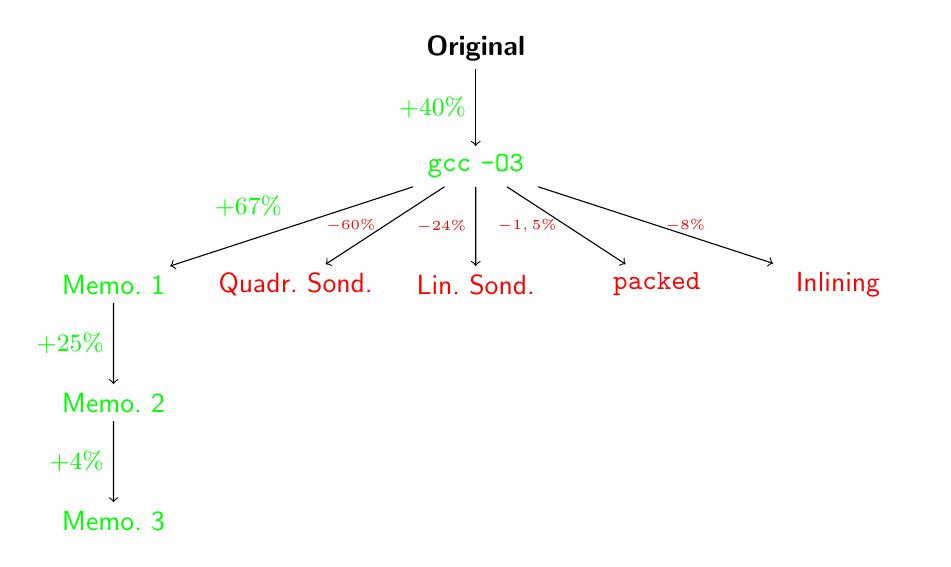
\begin{tikzpicture}[->,level/.style={sibling distance = 2.3cm,
  level distance = 1.5cm}]
    \node [arn_n] {\bfseries Original}
	child { node [arn_x] {\texttt{gcc -O3}}
		    child {
		      node [arn_x] {Memo.~1}
		      child {
			 node [arn_x] {Memo.~2}
			   child {
			     node[arn_x] {Memo.~3}
			     edge from parent node [left] {\small \success{$+4\%$}}
			   }
			 edge from parent node [left] {\small \success{$+25\%$}}
		      }
		      edge from parent node [above left] {\small \success{$+67\%$}}
		    }
		    child {
		      node [arn_r] {Quadr.~Sond.}
		      edge from parent node [left] {\tiny \fail{$-60\%$}}
		    }
		    child {
		      node [arn_r] {Lin.~Sond.}
		      edge from parent node [left] {\tiny \fail{$-24\%$}}
		    }
		    child {
		      node [arn_r] {\texttt{packed}}
		      edge from parent node [left] {\tiny \fail{$-1,5\%$}}
		    }
		    child {
		      node [arn_r] {Inlining}
		      edge from parent node [right] {\tiny \fail{$-8\%$}}
		    }
		    edge from parent node [left] {\small \success{$+40\%$}}
	}
    ;
\end{tikzpicture}
\end{center}
\end{frame}



\begin{frame}
  	\frametitle{Mathematischer Ansatz}
  	\framesubtitle{Aufl\"osung von Schleifen und explizite Darstellung}
  	\duploop
		

		Gleiche Berechnung (nur mit anderem Startwert) wird 10 mal durchgef\"uhrt.
\end{frame}

\begin{frame}
  	\frametitle{Mathematischer Ansatz}
  	\framesubtitle{Aufl\"osung von Schleifen und explizite Darstellung}
  	\diffgleichung
	
	\begin{block}{Differenzengleichung 1.~Ordnung}	
	$x_{n+1} = (x_{n} * 2654435761 + b_{n}) * (1 + \frac{1}{2^{32}})$
	\end{block}

	
\end{frame}

\begin{frame}
  	\frametitle{Mathematischer Ansatz}
  	\framesubtitle{Aufl\"osung von Schleifen und explizite Darstellung}
  	\diffgleichung
		
		$x_{n+1} = (x_{n} * 2654435761 + b_{n}) * (1 + \frac{1}{2^{32}})$

$x_{0} = 0$

$x_{1} = 0 * 2654435761 + b_{0} + \frac{x_{0}*2654435761 + b_{0}}{2 ^{32}} = b_{0} +  \frac{b_{0}}{2 ^{32}}  $

...

\end{frame}

\begin{frame}
  	\frametitle{Mathematischer Ansatz}
  	\framesubtitle{Aufl\"osung von Schleifen und explizite Darstellung}

$x_{2} = x_{1} * 2654435761 + b_{1} + \frac{x_{1}*2654435761 + b_{1}}{2^{32}}$

$x_{3} = ((b_{0} +  \frac{b_{0}}{2 ^{32}}) * 2654435761 + b_{1} + \frac{x_{1}*2654435761 + b_{1}}{2^{32}}) * 2654435761 + b_{2} + \frac{((b_{0} +  \frac{b_{0}}{2 ^{32}}) * 2654435761 + b_{1} + \frac{x_{1}*2654435761 + b_{1}}{2^{32}})*2654435761 + b_{2}}{2^{32}}$

...

\end{frame}

\begin{frame}
  	\frametitle{Mathematischer Ansatz}
  	\framesubtitle{Allgemeine iterative Berechnung von Differenzenglg. 1.~Ordnung}
	\begin{block}{vereinfachtes Beispiel:}
	
	
	$x_{n+1} = x_{n}* c + b_{n}$

	$x_{3} = ((x_{0} * c  + b_{0}) * c + b_{1}) * c + b_{2}$
	$x_{3} = c^3 * x_{0} + c^2 * b_{0} + c^1 * b_{1} + c^0 * b_{2}$
	$x_{n} = c^n * x_{0} + \sum_{i=0}^{n-1} c^{n-i-1} * b_{i}$
	\end{block}
	\begin{block}{Problematik:}
Man hat eine Potenz mit der \fail{Anzahl an Iterationen} als Hochzahl.\\
Bsp: input2 hat 724129 Zeilen \"uber die iteriert wird!
	\end{block}

\end{frame}

\end{document}
